% \documentclass[10pt, journal, compsoc, authoryear]{IEEEtran}
\documentclass[10pt, journal, compsoc, authoryear]{article}

% \setpagenumber{1}g
\usepackage{CJKutf8}


\usepackage{comment}

\usepackage[numbers]{natbib}

\usepackage{graphicx}
\usepackage{subfigure}
\usepackage{url}

\usepackage{amsthm}
\usepackage{amsmath}
 \numberwithin{equation}{subsection}
\usepackage{paralist}
\usepackage[pdfpagelabels]{hyperref}
\usepackage[all]{hypcap}
\usepackage{verbatim}
\usepackage{array}
\usepackage{float}
\usepackage{multirow}
% \usepackage{rotating}
\usepackage{multicol}
\usepackage{longtable}
\usepackage{graphicx}


\theoremstyle{definition}
\newtheorem{defn}{Definition}
\newtheorem{conj}{Conjecture}
%\newtheorem{exmp}{Example}[section]
\newtheorem{exmp}{Example}
\newenvironment{where}{\noindent{}where\begin{itemize}}{\end{itemize}}
% A comment in a draft (shouldn't appear in the final version).
\newcommand{\mycomment}[1]{\(\spadesuit\){\bf #1 }\(\spadesuit\)}
% Comment this out in the draft
% \newcommand{\mycomment}[1]{}
\newcommand{\pmcomment}[1]{\comment{PM}{#1}}
\newcommand{\pwtcomment}[1]{\comment{PT}{#1}}
\newcommand{\rscomment}[1]{\comment{RS}{#1}}

% line break in table.  e.g.
% Foo bar & \specialcell{Foo\\bar} & Foo bar \\    % vertically centered
% Foo bar & \specialcell[t]{Foo\\bar} & Foo bar \\ % aligned with top rule
\newcommand{\specialcell}[2][c]{%
  \begin{tabular}[#1]{@{}c@{}}#2\end{tabular}}

% \permission {[Copyright notice will appear here once ’preprint’ option is 
% removed.]}

\begin{document}


\title{Towards Precise Analysis for Software Rejuvenation \\ (v 0.1) } % title

\author{Jiansen HE}

% \category{I.3.7}{Computer Graphics}{Three-Dimensional Graphics and Realism}[Animation]
% \category{I.3.5}{Computer Graphics}{Computational Geometry and Object Modeling}[Physically based modeling]

% \terms{Experimentation, Human Factors}



\maketitle


\begin{comment} 
\begin{abstract} 

Software rejuvenation refers to a preventive failure recovery technique, which 
restarts a software regularly to reduce the cost of software ageing.  It has been  
actively studied in the literature and applied in enterprise level applications. 
Traditionally, a software system is modelled as a Semi-Markov process, from 
which a rejuvenation schedule is deducted to optimise the objective function 
(e.g. highest availability, lowest cost) after the system reaches its steady-state.
Unfortunately, it can takes a long time for a system to reach its steady-state.  
We propose a approximate simulation method to study XXX


Continue a line of work by \citet{huang1995software} and 
\citet{dohi2000statistical}, this paper proposes an alternative Markov 
model for software rejuvenate.  Specifically, we expend each state, $S$, in 
traditional models to a group of states, $S(\tau)$, where $\tau$ represents 
the elapsed time that the system has been entered into state $S$.  
The above model is equivalent to a semi-Markov process.  It, however, brings two 
benefits and one limitation.  The first 
benefit is that state transition probabilities can be precisely described.  
Like in general reliability studies, the failure rate in the new model 
can be precisely described by an arbitrary probability density function or 
probability mass function.  In contrast, traditional models either use the 
average Mean Time to Failure (MTTF) for cost analysis or assume that the time 
spent in each state has an exponential distribution.  The second 
benefit is that transition probabilities of the new Markov process has take 
time into account.  The result model is either a simple Markov chain if time is 
a discrete value,  or a general Markov process if time is a continuous value.  
Comparing to traditional models that are semi-Markov processes or Continuous 
Time Markov Chains (CTMT), the Markov Chain used in proposed model is often 
easier to understand and analysis.  The downside of expending the state space 
is the decreased performance of simulation processes.  Fortunately, approximate 
estimations can be given to balance the trade-off between accuracy and 
efficiency.  Most importantly, we show that the classical model given by 
\citep{huang1995software} is the least accurate approximation.  Moreover, 
inspired by economical theories, a notion of {\it utility} function
is proposes paper to unify the cost analysis and the availability 
analysis, which are usually treated separately in previous studies.



\end{abstract}
\end{comment} 

% \begin{IEEEkeywords}
% key1; key2; key3; 

% \end{IEEEkeywords}

% \IEEEpeerreviewmaketitle


\chapter{Introduction}

This introductory chapter presents the general background that motivates solving  problems discussed in this thesis.  It summarizes main contributions of this thesis.  Finally, an overview of the thesis is given.

\section{General Background and Motivation}

Building reliable distributed applications is among the most difficult tasks 
facing programmers, and one which is becoming increasingly important due to the 
recent advent of web applications, cloud services, and mobile apps.  Modern 
society relies on distributed applications which are executed on heterogeneous 
runtime environments, are tolerant of partial failures, and sometimes 
dynamically upgrade some of their components without affecting other parts.

A distributed application typically consists of components which handle some 
tasks independently, while collaborating on other tasks by exchanging
messages.  The robustness of a distributed application, therefore, 
can be improved by (i) using a fault-tolerant design to minimise the 
aftermath of partial failures, or (ii) employing type checking to detect 
some errors, including the logic of component implementations, and 
communications between components.

One of the most influential fault-tolerant designs is the supervision 
principle, proposed in the first release of the Erlang/OTP library in 1997 
\citep{OTP}. The supervision principle states that concurrent components of an 
application should be encapsulated as actors, which make local decisions in 
response to received messages.  Actors form a tree structure, where a parent 
node is responsible for monitoring its children and restarting them when 
necessary. The supervision principle is proposed to increase the robustness of 
applications written in Erlang, a dynamically typed programming language.  
Erlang application developers can employ the supervision principle by using 
related API from the Erlang/OTP library.  It is reported that the supervision 
principle helped AXD301, an ATM (Asynchronous Transfer Mode) switch 
manufactured by Ericsson Telecom AB. for British Telecom, to achieve 
99.9999999\% (9 nines) uptime during a nine-month test \citep{ArmstrongAXD}. 
Nevertheless, adopting the Supervision principle is optional in Erlang 
applications.

Aside from employing good design patterns, programmers can use typed 
programming languages to construct reliable and maintainable 
programs.  Typed programming languages have the advantages of detecting some 
errors earlier, enforcing disciplined and modular programming, providing 
guarantees on language safety, and efficiency optimisation \citep{TPL}.

Can programmers benefit from the advantages of both the 
supervision tree and type checking?  In fact, attempts have been made in two 
directions: statically type checking Erlang programs and porting the 
supervision principle to statically typed systems.

Static checking in Erlang can be done via optional checking tools or 
rewriting applications using an Erlang variant that uses a statically typed 
system.  Static analysis tools of Erlang include the Dialyzer \citep{Dialyzer} 
and a fault tolerance analysis tool by \citet{JanHenry}.  The Dialyzer tool is 
shipped with Erlang.  It has identified a number of unnoticed errors in large 
Erlang applications that have been run for many years 
\citep{DialyzerDetecting}. Nevertheless, the use of Dialyzer and other 
analysis tools is often involved in the later stages of Erlang applications 
development.  In comparison with static analysis tools, simplified Erlang 
variants that use static type systems have been designed by 
\citet{marlow1997practical}, \citet{sabelfeld2002securing}, among others.  As 
the expressiveness is often sacrificed in those simplified variants to some 
extent, code modifications are more or less required to make existing 
Erlang programs go through the type checker.

The second attempt is porting the notion of actors and supervision trees to 
statically typed languages, including Scala and Haskell.  Scala actor 
libraries, 
including Scala Actors \citep{actor_1, actor_2} and Akka 
\citep{akka_api,akka_doc}, use 
dynamically typed messages even though Scala is a statically typed language.  
Some recent actor libraries, including Cloud Haskell \citep{CloudHaskell}, Lift 
\citep{lift_scala}, and scalaz \citep{scalaz}, support both 
dynamically and statically typed messages, but do not support supervision.  Can 
actors in supervision trees be statically typed? 

The key claim in this thesis is that actors in supervision trees can be 
statically typed by parameterizing the actor class with the type of messages it 
expects to receive.  This research project is motivated by the following benefits of statical typing:
\begin{enumerate}
  \item Both users and developers of actor-based services can take advantages 
of type-parameterized actors.  For users, sending ill-typed messages is 
prevented at compile time.  Because messages are usually transmitted 
asynchronously, it may be otherwise difficult to trace the source of errors at 
runtime, especially in distributed environments.  For service developers, since 
unexpected messages are eliminated from the system, they can focus on the 
logic of the services rather than worrying about incoming messages of 
unexpected types.  Another immediate benefits of typing checking is pattern
completeness checking for message handlers.
  \item Static typing enforces disciplined and modular programming \citep{TPL}.
Opposite to writing programs in dynamically typed languages, programers are often more confident to use complex and deep nested types in statically typed languages.  Using complex types that have a higher level of abstraction improves the readability and maintainability of programs.  On the other side, porting nested types into an untyped system using nested tuples is possible but often results in complex code that is more difficult to understand.
  \item Static typing often results in shorter code \citep{TPL}.  When a new actor is defined, handlers for ill-typed messages are no longer needed.  When an application is built on top of some actors, which are often black boxes to application developers, there is no need to study how those actors will behave upon receiving unexpected messages and implement handlers for every problematic cases.
  \item A statically typed program can often be compiled to code that executes more quickly \citep{TPL}.  As the compiler knows the exact data types that are in use at runtime, ad hoc optimizations might be applied to the assembly code or the machine code.
  \item Statically typed interface is a clear and precise documentation per se \citep{TPL}.  Users of a type-parameterized actor understands its functionality immediately by looking at its type parameter, which denotes the type of permitted messages.  Without the type information, users would be more rely on good documentation, examples, and even small experiments created by themselves\citep{endrikat2014api}.

\end{enumerate}


Implementing type-parameterized actors in a statically-typed language, however, 
requires solving the following three problems:

\begin{enumerate}
  \item A typed name server is required to retrieve actor references of
specific types.  A distributed system usually requires a name server which
maps names of services to processes that implement that service.  If processes
are dynamically typed, the name server is usually implemented as a map from 
names to processes. Can a distributed name server maintain maps from the typed 
names and processes of corresponding types, and provide API for 
registering and fetching statically typed processes?

  \item A supervisor actor must interact with child actors of different types. 
Each actor in a supervision tree needs to handle messages for both the purpose 
of supervision and its own specific interests.  When all actors are 
parameterized by different types, is it practical to define a supervisor that 
communicates with children of different types?

  \item Actors that receive messages from distinct parties may suffer from the 
type pollution problem, whereby a party imports too much type information 
about an actor and can send the actor messages not expected from it. Systems 
built on a layered architecture or the MVC model are often victims of the type 
pollution problem. As an actor receives messages from distinct parties using its 
sole channel, its type parameter is the union type of all expected message 
types. Therefore, unexpected messages can be sent to an actor which naively 
publishes its type parameter or permits dynamically typed messages. Can a 
type-parameterized actor publish itself as different types when it communicates 
with different parties?
\end{enumerate}

\section{Contributions}

The overall goal of the thesis is to develop a framework that makes it possible 
to construct reliable distributed applications written using and validated by 
our library, TAkka, which merges the advantages of type checking and the 
supervision principle.   

The TAkka library is implemented in the Scala programming language.  It
expands the existing Akka library for supervised actors by the introduction 
of typed messaging.  Akka is developed at TypeSafe Inc.  
As Akka becomes part of the standard library in Scala 2.10 
and higher versions, it is widely used in many real applications.  Choosing 
Akka as the base of our design and implementation benefits this project in 
many aspects.  Firstly, the author checks that main requirements in distributed 
programming are not unintentionally neglected by rewriting 23 Akka applications 
written by other professional programmers.  Secondly, improvements made in 
the TAkka library can benefit existing Akka applications with a low cost because, 
as presented later, rewriting Akka applications using TAkka involves less than 10\% 
straightforward code changes.  Finally, despite some deficits in the Akka design, 
it saves the author a significant amount of work on low-level implementation.  
In fact, some less carefully designed Akka features have inspired the author to 
make improvements in the TAkka library.

Source code of the TAkka library, testing and demonstration examples, along with
other related documentations produced during this research are available at a 
GitHub repository for this project \citep{takka_repo} and the CD attached to this thesis.
A condensed version of the material in this thesis is published in a companion paper \citep{TAKKA_paper}.

Generally speaking, the key contributions of this thesis are:

\begin{itemize}
\begin{comment}
  \item A formal model that captures the essence of the supervision principle.  
  The model (Chapter~\ref{supervision_model}) exhibits key features of the 
  supervision principle used in existing libraries including Erlang, Akka, and 
  TAkka. It provides a tool to compare the design alternatives to the 
  supervision principle.  
\end{comment}  
  \item The design and implementation of the TAkka library (Chapter~\ref{takka_design}), where supervised 
actors are parameterized by the type of messages they expect.  The library 
  mixes static and dynamic type checking so that type
  errors are detected at the earliest opportunity.  The library separates 
  message types and message handlers for the purpose of supervision from those 
  for actor specific communications.  The decision is made so that   
  type-parameterized actors of different types can form a supervision tree. 
%  Interestingly, this decision coincides with our recommendation in the model 
%  analysis for improving availability.  
  Chapter~\ref{evolution} shows that Akka 
  programs can be upgraded to their TAkka equivalents incrementally, one module 
  at a time (evolution), rather 
  than requiring a monolithic change to all modules simultaneously (revolution).  The
  design is analogous to a design principle of Java Generics, known as ``Evolution,
  not Revolution''

  
  \item A framework for evaluating libraries that supports the supervision 
  principle. Chapter~\ref{takka_evaluation} shows that the type pollution 
  problem can be straightforwardly avoided in TAkka.  The evaluation further 
  compares the TAkka library and the Akka library in terms of expressiveness, efficiency and 
  scalability. Results show that TAkka applications add minimal runtime overhead 
  to the underlying Akka system and have a similar code size and scalability 
  compared with their Akka equivalents. Finally, TAkka ports the Chaos Monkey 
  library and design a Supervision View library.  The Chaos Monkey library tests whether 
  exceptions are properly handled by supervisors.  The Supervision View library 
  dynamically captures the structure of supervision trees. We believe that similar 
  evaluations can be done in Erlang and new libraries that support the supervision 
  principle.
\begin{comment}  
  \item A model for analyzing the reliability and availability of 
  fault-tolerant systems that use the {\it reactive} mechanism (supervision) 
  and the {\it proactive} mechanism (software rejuvenation).  The novel model 
  (Chapter~\ref{rejuvenation_model}) overcomes the limitation of the classic 
  software rejuvenation model where the failure rate is treated as a constant
  and failure recovery is ironically treated as a stochastic process.  
  \mycomment{add new contributions once achieved}
  \mycomment{efficient approximate estimation}
  \mycomment{? the classic model is the least accurate approximation. ?}  
\end{comment}  
\end{itemize}

\section{Thesis Outline}

The rest of this thesis is structured as the followings.

Chapter~\ref{background} summarises work that influences the design and implementation
of the TAkka library.  It introduces elements of the Actor Programming model and the 
Supervision principle, together with short explanations of their usages in the Erlang 
language and the Akka library.  Chapter~\ref{background} concludes with features of the
Scala type system used in the TAkka implementation.   

A condensed version of the material in Chapter~\ref{takka_design} to \ref{takka_evaluation}
appears in a companion paper.  The paper \citep{TAKKA_paper} 
is written as a brief introduction to the TAkka library.  It
is structured in a way that make the comparison of TAkka and Akka easy for Scala programmers.
This thesis elaborates the rational for the TAkka design and implementation.   
Chapter~\ref{takka_design} presents the design and implementation of the TAkka library. 
Chapter~\ref{evolution} shows that Akka programs can be rewritten using TAkka incrementally, 
one module at a time.  Chapter \ref{takka_evaluation} evaluates the TAkka library.

Chapter~\ref{summary} concludes and suggests future work that can help the construction of reliable
distributed applications. 

\section{Background}


\subsection{Basic Failure Model in Reliability Study}

In reliability study, the time when the first failure occurs in often assumed 
to follow a probability density function (pdf) if time is a continuous value, or 
a probability mass function (pmf) if time is a discrete value. \citep{MusaBook} 
 
The value of time is a continuous value if its unit is a {\it time unit} (e.g. 
second) and the value could be any real number.  The value of time is 
a discrete value if its unit is a {\it natural unit} (e.g. number of 
operations) or its unit is a {\it time unit} but the user only cares the 
status of a system at discrete time (e.g. every second).

Although the precise definition of failure varies in different systems, 
measures of failures can be consistently defined in terms of a pdf or a
pmf.  Assuming that the pdf of a system is $f(t)$, measures of failures can be 
defined as in Figure \ref{eq:measure_of_failures} 
\citep{MusaBook}.  Measures of failures can be defined in terms of pmf 
similarly.

\begin{figure}
\begin{subequations} 
\begin{align}
    R(t) & = \int_{t}^{\infty} f(x) dx = 1- \int_{0}^{t} f(x) dx  \label{subeq1}\\
   MTTF & = \int_{0}^{\infty} tf(t)dt  = \int_{0}^{\infty} R(t)dt 
\label{mttf}\\
   h(t) & = \lim_{\Delta t\rightarrow 0} \frac{R(t)-R(t+\Delta t)}{\Delta t 
R(t)}  = \frac{f(t)}{R(t)}
\end{align}
\end{subequations}
\caption{Measures of Failures}
\label{eq:measure_of_failures}
\end{figure}

In the above, the reliability during a specific time, $R(t)$, is the 
probability that a system can survive without failure throughout that time.  
The Mean Time to Failure (MTTF) is the average time when the first failure 
occurs.  The hazard rate at time $t$ is the failure rate at that time given 
the condition that the system has survived for $t$ time.  Equation 
\ref{failure_check} checks that the average failure rate ($\lambda$) is the 
reciprocal of MTTF.

\begin{equation}
 \lambda = \int_{0}^{\infty} h(t) dt = \int_{0}^{\infty} \frac{f(t)}{R(t)}  dt 
=  \frac{\int_{0}^{\infty} f(t) dt}{\int_{0}^{\infty} R(t) dt} = \frac{1}{MTTF}
\label{failure_check}
\end{equation}




\subsection{Traditional Software Rejuvenation Models}

\subsubsection{The Basic Model}


The basic software rejuvenation model proposed by
\citep{huang1995software} is modelled by the state transition diagram in 
Figure \ref{fig:model_classic_1}.  Huang et. al defines the following 4 states:

\begin{description}
  \item[S] The robust {\tt start} state in which the system will not fail.
  \item[W] The failure probable {\tt working} state in which the system may 
fail at a certain probability.
  \item[F] The {\tt failure} state when the system reaches its boundary condition.
  \item[R] The {\tt rejuvenation} state when the system is plan to 
restart to a clean state.
\end{description}

\citep{huang1995software} decides the rejuvenation thresholds using the 
following process.  

\begin{enumerate}
  \item compute the probabilistic {\it mean} rates of every state transitions 
somehow.
  \item calculate the probability of the system being in each state, based on 
the state transition rates computed above.
  \item calculate the {\it expected} total time of the system in state $s$ 
during an interval of $L$ time units as $T_s(L) = p_s \times L$, where $p_s$ is 
the probability the system being in state $s$ calculated in the second step.
  \item calculate the cost of downtime during interval $L$ as $Cost(L) = (p_f 
\times c_f + p_r \times c_r) \times L$, where $p_f$ and $p_r$ are probabilities 
the system in state $F$ and $R$ respectively, and $c_f$ and $c_r$ are unit cost 
of the system in state $F$ and $R$ respectively.
  \item determine the optimal rejuvenation thresholds by finding the optimal 
transition rate between state $W$ to state $F$ so that the cost of downtime is 
minimum.
\end{enumerate} 

The original software rejuvenation model, proposed by 
\citet{huang1995software}, has shown its significance in long running billing 
systems, scientific applications, and telecommunication systems 
\citep{huang1995software}. Readers may have noticed that the above estimation 
methodology gives an approximate statistical estimation for a long running 
system because the usage of {\it mean} state transition rates and the {\it 
expected} time of being in each state.  By {\it long running system}, we refer 
to a system whose expected in-service time is a statistically long time regards 
to its MTTF, repair time, and rejuvenation time.


\begin{figure}
  \centering         
        \subfigure[Traditional Model 1]{
            \label{fig:model_classic_1}
            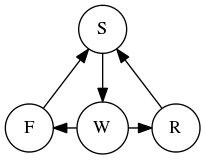
\includegraphics[scale=0.5]{model_1.png}
        }\\
        \subfigure[Traditional Model 2]{
            \label{fig:model_classic_2}
            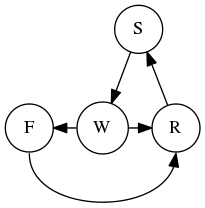
\includegraphics[scale=0.5]{model_2.png}
        }\\
    \caption{Traditional Software Rejuvenation Models}
   \label{fig:model_traditional}
\end{figure}

\subsubsection{A Modified Model}

\citet{dohi2000statistical} modifies the original model given 
by \citet{huang1995software} with the following modifications:

\begin{enumerate}
  \item As shown in Figure \ref{fig:model_classic_2}, the completion of repair process
  is immediately followed by the software rejuvenation process.
  \item Assuming that every state transition is a stochastic processes.  For each state $S$, define a 
  probability density function $F_s(t)$, which represents the probability that the system will stay in that
  state for time $t$. 
\end{enumerate} 

The first modification is made to distinguish the process of system cleanup and process resuming
from other repair tasks, the former of which is required in both the repair process and the rejuvenation
process in practice.  The second assumption is made so that the model is a Semi-Markov process,
a well studied stochastic process with off-the-shelf analysis techniques.  Although \citet{huang1995software}
do not mention the relationship between their model and Markov process, \citet{dohi2000statistical}
show that if the modified model gives the same analysis result as the one
given in \citet{huang1995software} if (i) remove assumption 1; and (ii) assume 
that the sojourn times in all states are exponentially distributed.

\citet{dohi2000statistical} decides the optimal software rejuvenation thresholds by looking for
the one that maximise the system availability, the ratio of uptime and total time.  Same as the
methodology in \citet{huang1995software}, instead of precisely describe state transition 
probabilities, $mean$ time of staying in the {\tt start} state, the {\tt failure} state, and the
{\tt rejuvenation} state is used.  The expected time of staying the failure probable {\tt working} state
is calculated by equation \ref{mttf}.

The methodology given in \citet{dohi2000statistical}  does not give a general cost
analysis as the one in \citet{huang1995software}.  It also suffers the problem of using
$mean$ times.  Despite those two limitations, \citet{dohi2000statistical} 
derived a non-parametric statistical algorithms to estimate the optimal 
software rejuvenation thresholds that maximise the system availability, based 
on statistical complete sample data of failure times.



\begin{comment}
The basic assumption of software rejuvenation is that software systems will 
become failure-probable after a period of execution.  In other words, failure 
rate is a function about the execution time t.  In contrast, the probabilistic 
state transition model 
\url{
http://citeseerx.ist.psu.edu/viewdoc/download?doi=10.1.1.176.2557&rep=rep1&type=
pdf} (FTCS 1995, citation: 711) employs the statistical mean rate of the 
transition rate between states.  

   The same model is used in the book 
\url{http://onlinelibrary.wiley.com/doi/10.1002/9780470050118.ecse394/full} 
(published in 2007)

   The same problem appears in the model used in 
\url{http://ieeexplore.ieee.org/xpls/abs_all.jsp?arnumber=897287} (HASE 2000, 
citation: 60) and 
\url{http://ieeexplore.ieee.org/stamp/stamp.jsp?tp=&arnumber=895436} (PRDC 2000, 
citation: 90), which extends the original model to be a semi-Markov process, 
where time is a continuous value.
      

Models that use the statistical mean rate can only be used to estimate the 
expected average behaviors (e.g. downtime) over a statistically long time.  A 
more serious problem is that, treating failure rate as a constant in model 
analysis violates the basic assumption of software rejuvenation.  After all, if 
the failure rate is independent of the execution time, restarting the system 
will not help at all but increase the downtime.

The link ( http://srejuv.ee.duke.edu/papers.htm ) gives a list of papers (until 
2010) on software rejuvenation.  I am surprised that the classic general failure 
model used in reliability analysis has not been applied to the model analysis of 
software rejuvenation.
\end{comment}

\section{A New Model}

\subsection{Definitions}

To overcome the limitations of classical models, which focus on the 
equilibrium status that will take a long time to reach, this paper propose a
new model that enables effective simulation on early-stages of a system using 
rejuvenation.  The new model works as the follows. It is initialised to a 
working state and its {\it software rejuvenate schedule} is set to time $T$.  
The failure rate during the working period is a function of the elapsed working 
time $t$.  A failed system takes $t_f$ time to repair.  At the end of a repair 
process or after working for $T$ time, the system enters to the rejuvenation 
process for $t_r$ time before being set to the initial working state.  Figure 
\ref{model_new} gives the transition digram for the new Model, which consists 
of  the following 3 {\it categories} of states:

\begin{itemize}
 \item {\tt W($\tau$), $0 \leq \tau < T$} the state that the system has running 
without failure for $\tau$ time;
 \item {\tt R($\tau$), $0 \leq \tau < t_r$} the state that the system has 
entered 
the rejuvenation process for $\tau$ time.
 \item {\tt F($\tau$), $0 \leq \tau < t_f$} the state that the system has 
failed 
for $\tau$ time, during which period no rejuvenation process has been invoked, 
but other repair processes, such as data restore, maybe performed.
\end{itemize}

For the convince of later discussions, this paper index possible state $x_i$ as 
follows:

\begin{defn}
\[ x_i = \left\{ 
  \begin{array}{l l}
    W(i)    &   0 \leq i < T \\
    R(i-T) &   T \leq i < T+t_r \\ 
    F(i-T-t_r) &   T+t_r \leq i < T+t_r+t_f \\     
  \end{array} \right.\]
\end{defn}

Let $X_t$ be the state of the system at time $t \geq 0$, then the process $X = 
(X_t, t \geq 0)$ is a stochastic process.  If time is a discrete value in the 
model, the process has discrete time and discrete state space.  
If time is a  continuous value in the model, the process has 
continuous time and continuous state space.  




\begin{figure}
  \label{model_new}
  \centering       
  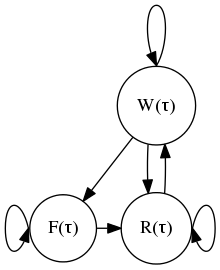
\includegraphics[scale=0.5]{model.png}
  \caption{New Model}
\end{figure}


\subsection{Cast Continues State Space to Discrete State Space}

As Section \ref{discrete_model} will show, a standard Markov Chain can be 
defined if time is treated as a discrete value.  Section 
\ref{discrete_simulation} will give the simulation process corresponding to 
the Markov Chain.  Although a general Markov process can be defined similarly 
for the case where time is a continuous value, unfortunately, the general 
Markov process does not have a precise simulation method.  Therefore, this 
paper converts the continuous case to an approximate discrete case, where a 
simulation method can be applied.  

To convert a model with continuous state space to one with discrete state space,
a new time unit, $\Delta t >  0$, is picked such that 
$T/\Delta t$, $t_r/\Delta t$, and $t_f/\Delta t$ are integers.  Let $pdf$ be 
the failure density function in the continues model, then the failure massive 
function at $T+\Delta t$ in the discrete model is 

\begin{equation}
pmf(T+\Delta t) =  \int_{T}^{T+\Delta t} pdf(t) dt
\end{equation}

Finally, times $t$ in the continuous model can be converted to $t/\Delta t$ in 
the new discrete model.

\begin{comment}
\subsubsection{The Transaction Probability Density}

Let $p_{ij}$ be the probability of moving from $X_i$ to $X_j$ and $0 \le j-i 
\le 
min\{T, t_r, t_f\}$.  
We have:

\begin{equation}
p_{ij} = 
\begin{cases} 
\frac{R(k+j-i)}{R(k)}    &  if\ x_i = W(k), \\ &\hspace{12pt}  x_j = W(k+j-i), 
\\ &\hspace{12pt}  0\leq k <T+i-j; \\

\frac{R(T)}{ R(k)}     &  if\ x_i = W(k),   x_j = F(l), \\ &\hspace{12pt}  
0\leq 
k < T, 0 \leq l < j-i; \\ 

\frac{R(T)}{R(k)}     &   if\ x_i = W(T-k),   x_j = R(k),\\ &\hspace{12pt}   0 
\leq k < j-i; \\

\int_{0}^{w} f(x)dx     &  if\ x_i = R(k),   x_j = F(l), \\ &\hspace{12pt}  
0\leq k < t_r, 0 \leq l < t_f; \\ &\hspace{12pt}  w = (j-i)-(t_r-k)-(t_f-l) \\

1     &  if\ x_i = R(k),  x_j = R(k+j-i),\\ &\hspace{12pt}   0\leq k <t_r+i-j, 
\\
       &  or\ x_i = F(k),   x_j = F(k+j-i),\\ &\hspace{12pt}   0\leq k 
<t_f+i-j, 
\\     
       &  or\ x_i = F(t_f-k),   x_j = R(k),\\ &\hspace{12pt}   0 \leq k < t_r, 
\\      
       &   or\ if\ x_i = R(t_r-k), \\ &\hspace{12pt}  x_j = W(k),   0 \leq k < 
T; \\       
0     &   otherwise
\end{cases}
\end{equation}
\hspace{90pt} where $0 \le j-i \le min{T, t_r, t_f}$
\end{comment}


\subsection{Discrete Model as a Markov Chain}
\label{discrete_model}

\subsubsection{Probability Mass Function and Failure Rate}

Let $f(t)$ be the probability mass function (pmf) which represents the 
probability that, without software rejuvenation, the system will fail when 
being running for exactly $t$.  We can derive its reliability function ($R(t)$) 
and the failure rate function ($\lambda(t)$) as follows:

\begin{subequations}
\begin{align}
R(t) & = 1- \sum \limits_{i=1}^{t-1} f(t) & t > 0 \label{discrete_reliability}\\
\lambda(t) & = f(t)/R(t)  & t>0 \label{discrete_failure_rate}
\end{align}
\end{subequations}

Intuitively, $R(t)$ is the probability that the system can survive for as least 
$t$ time and $\lambda(t)$ is the probability that the system, which has 
survived for time $t$, fails at the next moment.

\subsubsection{The Transaction Matrix}

We define the transaction matrix $P$ whose $(i,j)$th element is the probability 
of moving from $x_i$ to $x_j$ in exactly {\it one} unit of time,  we have:

\begin{equation*}
p_{ij} = 
\begin{cases} 
1 - \lambda(k) & if\ x_i = W(k), x_j = W(k+1),\\ &\hspace{12pt}  0\leq k <T-1; 
\\
\lambda(k)     & if\ x_i = W(k), x_j = F(0),\\ &\hspace{12pt}  0\leq k <T-1,  \\
1              & if\ x_i = W(T-1), x_j = R(0), \\
               & or\ x_i = R(k), x_j = R(k+1),\\ &\hspace{12pt}  0\leq k < 
t_r-1, \\
               & or\ x_i = R(t_r), x_j = W(0), \\
               & or\ x_i = F(k), x_j = F(k+1),\\ &\hspace{12pt}  0\leq k <t_f-1, 
\\
               & or\ x_i = F(t_f), x_j = R(0); \\
0              & otherwise
\end{cases}
\end{equation*}

It is easy to verify that $P$ satisfies the following two properties of {\it stochastic matrix}:
\begin{enumerate}[\itshape a\upshape)]
\item $p_{ij} \ge 0$, and
\item $\sum \limits_{i} p_{ij} = 1$.
\end{enumerate}



\subsubsection{Simulation}
\label{discrete_simulation}

Let $\mu_t$ be a row vector of probabilities so that $\mu_t(i)$ represents the 
probability that the system is at state $x_i$ at time $t$, we can inductively 
simulate $\mu_t$ as the follows:

\begin{subequations}
\label{discrete_simulation_mu}
\begin{align}
\mu_0 & =  \begin{cases}  \mu_0(0) = 1 & \\
    \mu_0(i) = 0 & 0 < i < T+t_r+t_f -1
\end{cases}  \label{mu_0}\\
\mu_t & = \mu_0 P  &  \label{mu_t}
\end{align}
\end{subequations}
Particularly, a row vector $\pi$ is called a stationary distribution if $\pi = 
\pi P$.

On the other hand, the Chapman-Kolmogorov Equation states the follows:

\begin{equation}
\label{discrete_CK}
p_{ij}(m+n) = \sum \limits_k p_{ik}(m)p_{kj}(n)
\end{equation}

where $p_{ij}(n)$ is the probability that the system moves from state $X_i$
to state $X_j$ with in exactly $n$ steps.  

A nice corollary of Equation \ref{discrete_CK} is:
\begin{equation}
\label{discrete_CK_corollary}
P_n = P^n
\end{equation}
where $P_n$ is the transaction matrix whose $(i,j)$th element is the probability 
of moving from $x_i$ to $x_j$ in exactly $n$ unit of time.

From either Equation \ref{discrete_simulation_mu} or Equation 
\ref{discrete_CK_corollary}, we have
\begin{equation}
\label{discrete_CK_corollary}
\mu_t = \mu_0 P^t
\end{equation}
a standard property of (time-homogeneous) Markov Chain.



\subsubsection{Utility Analysis}

Borrowed from economics, the notion of utility function is used to unifies
downtime cost analysis, availability analysis, and other variants in literature.

Let $u(i)$ be {\it utility function} that returns a real value if the system stays
at state $x_i$ for one unit of time, the $expected$ utility gained at time $t$,
and the $total$ utility gained until time $t$ are Equation \ref{discrete_utility_t}
and Equation \ref{discrete_utility_T} respectively.

\begin{subequations}
\label{discrete_utility}
\begin{align}
u_t  & =   \sum \limits_{i=0}^{T+t_r+t_f-1} u(i)\mu_t(i)  \label{discrete_utility_t}\\
U_t  & =  F_{i=0}^{t} u_i  \label{discrete_utility_T}
\end{align}
\end{subequations}
where $F$ is an accumulating function.


\newpage
CASE I: Availability Analysis

The utility function for availability analysis can be defined as:

\begin{equation}
\label{discrete_availability_utiliy}
u(i) =  \begin{cases}  1 & 0 \leq i < T \\
                       0 & T \leq i < T+t_r+t_f -1
\end{cases}
\end{equation}


The target of \citep{dohi2000statistical} is finding a value $T$ so that
$a = \sum \limits_{i=0}^{T+t_r+t_f-1} u(i)\pi(i) $ has a maximum value.
Notice that, the changes of systems availability before the Markov model 
reaches its steady-state $\pi$ is ignored in \citep{dohi2000statistical}.

For a safety crucial system expected to run $t$ time, users may want to use the 
following objective function instead.

\begin{equation}
\label{discrete_availability_minimum}
A_{min}(t) = \min_{i=0}^t u_i
\end{equation} 

The average availability of a system during its first $t$ time is:

\begin{equation}
\label{discrete_availability_average}
\bar{A}(t) = \frac{1}{ t }\sum \limits_{i=0}^{t} u_i
\end{equation}

If the system can reaches its steady-state $\pi$, one may expect that 
\begin{equation}
  \lim_{t\rightarrow \infty}{\bar{A}(t)} = a
\end{equation}

CASE II: Downtime Cost Analysis

As in \citep{huang1995software}, let $c_f$ and $c_r$ be the unit cost 
of the system in state $F$ and $R$ respectively, we have:

\begin{equation}
\label{discrete_downtime_utiliy}
u(i) =  \begin{cases}   0 & 0 \leq i < T \\
                       -c_r & T \leq i < T + t_r \\
                       -c_f & T + t_r \leq i < T + t_r + t_f
        \end{cases}
\end{equation}

The target of \citep{huang1995software} is finding a value $T$ so that
$c = \sum \limits_{i=0}^{T+t_r+t_f-1} u(i)\pi(i) $ has a maximum value.
Notice that, the changes of systems availability before the Markov model 
reaches its steady-state $\pi$ is ignored in \citep{dohi2000statistical}.
Actually, the expected total cost of running the system for $L$ time is:
\begin{equation}
\label{discrete_availability_total}
C(L) = \sum \limits_{t=0}^{L} u_t
\end{equation}

Only when the system can reaches its steady-state $\pi$, , one may expect 
that 
\begin{equation}
  \lim_{L\rightarrow \infty}{C(L)} = cL
\end{equation}

\newpage

CASE III: Benefit Analysis

The utility function in CASE I returns non-negative value while the utility 
function in CASE II returns non-positive value.  In reality, a software 
application gains revenue when it runs and cost resources to restart it when it 
is down.

Now consider an international Voice over Internet Protocol (VoIP) service 
provider, who implements a few independent front-end applications, each of 
which has the following utility function, where the unit of time is hour:

\begin{equation}
\label{discrete_benifit_utiliy}
u(i) =  \begin{cases}     r & 0 \leq i < T \\
                       -c_r & T \leq i < T + t_r \\
                       -c_f & T + t_r \leq i < T + t_r + t_f
        \end{cases}
\end{equation}

The goal is set a proper rejuvenation schedule $T$ to maximize the total 
utility gained during the expect service time $L$ defined as: 
\begin{equation}
\label{discrete_benifi_total}
U(L) = \sum \limits_{t=0}^{L} u_t = \sum \limits_{t=0}^{L}  \sum 
\limits_{i=0}^{T+t_r+t_f-1} u(i)\mu_t(i)
\end{equation}


\subsection{Reflection on Markov Processes}

The model in \citep{huang1995software} has its root in Continuous Time Markov 
Chain.  The model in \citep{dohi2000statistical} is a Continuous Time 
Semi-Markov Chain. Our model is a devised Discrete Time Markov Chain (DTMC) or 
a General Markov Process.

The General Markov Process is a precise model for software rejuvenation, but it 
may not have an analysitcal form for the simulation purpose.  Our devised 
DTMC adds a time parameter to standard DTMC, result in a special form of CTMC 
and SMC.

The problem of our devised DTMC is the expanded state space. Recall that the 
simulation process, $\mu_t = \mu_{t-1} P$, computes the product of a $1 \times 
n$ matrix and a $n \times n$ matrix, where $n$ is the number of states in the 
model.  It appears that the computational cost of the simulation 
process of the devised DTMC is impractical in a general case where $n$ is a 
large number.

Fortunately, the devised DTMC is an acceptable model for the software 
rejuvenation problem discussed in this paper for two reasons.  Firstly, 
non-zero values in the state transition matrix are sparsely distributed, and 
therefore matrix multiplication does not necessary require a long time to 
compute.   Secondly, similar to the process of reducing a continuous model to a 
discrete model, the state space of a descrete model can be further reduced for 
achieving better performance, with the cost of sacrifying accuracy.
\section{Numerical Illustrations}

\subsection{Examples from \citep{huang1995software}}

\subsubsection{Example A}
\begin{itemize}
  \item Mean Time Between Failures (MTBF): $12 \times 30 \times 24$ hours
  \item failure repair time:  30 minutes
  \item base longevity interval:  $7 \times 24$ hours
  \item rejuvenation time: 20 minutes
  \item average cost of unscheduled downtime: \$1700 / hour
  \item average cost of scheduled downtime: \$40 / hour  
\end{itemize}

\begin{table}[h]
\begin{tabular}{ | l || c | c | c | }
  \hline
   \multicolumn{4}{|c|}{For $12 \times 30 \times 24 $ hours } \\
  \hline                       
    & no rejuvenation & once every 3 weeks & once every two weeks \\
   \hline     
  Hours of Down Time  & 0.49 & 5.965 & 8.727 \\
  \hline    
  \$Cost of Down Time & 490  & 554 & 586 \\
  \hline 
\end{tabular}
  \caption{Huang etc's estimation for Example A}
\end{table}  
  


\subsubsection{Example B}
\begin{itemize}
  \item Mean Time Between Failures (MTBF): $3 \times 30 \times 24$ hours
  \item failure repair time:  30 minutes
  \item base longevity interval:  $3 \times 24$ hours
  \item rejuvenation time: 10 minutes
  \item average cost of unscheduled downtime: \$5000 / hour
  \item average cost of scheduled downtime: \$5 / hour  
\end{itemize}

\begin{table}[h]
\begin{tabular}{ | l || c | c | c | }
  \hline
   \multicolumn{4}{|c|}{For $12 \times 30 \times 24 $ hours } \\
  \hline                       
    & no rejuvenation & once every 2 weeks & once a week \\
   \hline     
  Hours of Down Time  & 1.94 & 5.70 & 9.52 \\
  \hline    
  \$Cost of Down Time & 9675.25  & 7672.43 & 5643.31 \\
  \hline  
\end{tabular}
  \caption{Huang etc's estimation for Example B}
\end{table}  
  

\begin{figure}[h]
     \begin{center}
     \subfigure[]{
\includegraphics[scale=0.18]{./plot/Huang1995B2/accumulated_cost_day.png}
        }
\subfigure[]{
\includegraphics[scale=0.18]{./plot/Huang1995B2/accumulated_cost_month.png}
        }\\
        \subfigure[]{            
\includegraphics[scale=0.18]{./plot/Huang1995B3/accumulated_cost_day.png}
        }
	\subfigure[]{            
\includegraphics[scale=0.18]{./plot/Huang1995B3/accumulated_downtime_month.png}
        }\\ 
        
        \subfigure[]{
\includegraphics[scale=0.18]{./plot/Huang1995B2/availability_day.png}
        }
\subfigure[]{
\includegraphics[scale=0.18]{./plot/Huang1995B2/availability_month.png}
        }\\
        \subfigure[]{            
\includegraphics[scale=0.18]{./plot/Huang1995B3/availability_day.png}
        }
	\subfigure[]{            
\includegraphics[scale=0.18]{./plot/Huang1995B3/availability_month.png}
        }\\ 
        
             \subfigure[]{
\includegraphics[scale=0.18]{./plot/Huang1995B2/acc_rej_time_day.png}
        }
\subfigure[]{
\includegraphics[scale=0.18]{./plot/Huang1995B2/acc_rej_time_month.png}
        }\\
        \subfigure[]{            
\includegraphics[scale=0.18]{./plot/Huang1995B3/acc_rej_time_day.png}
        }
	\subfigure[]{            
\includegraphics[scale=0.18]{./plot/Huang1995B3/acc_rej_time_month.png}
        }\\

    \end{center}
     \caption{Example B}
   \label{throughput}
\end{figure}

\subsubsection{Example C}
\begin{itemize}
  \item Mean Time Between Failures (MTBF): $3 \times 30 \times 24$ hours
  \item failure repair time:  $2$ hours
  \item base longevity interval (BLI):  $10 \times 24$ hours
  \item rejuvenation time: 10 minutes
  \item average cost of unscheduled downtime: \$5000 / hour
  \item average cost of scheduled downtime: \$5 / hour  
\end{itemize}

\begin{table}[h]
\begin{tabular}{ | l || c | c | c | }
  \hline
   \multicolumn{4}{|c|}{For $12 \times 30 \times 24 $ hours } \\
  \hline                       
    & no rejuvenation & once every 2 weeks & once a week \\
   \hline     
  Hours of Down Time  & 7019 & 6.83 & 6.36 \\
  \hline    
  \$Cost of Down Time & 3.6K  & 2.48K & 1.11K \\
  \hline  
\end{tabular}
  \caption{Huang etc's estimation for Example C}
\end{table}  
  

\begin{figure}[h]
     \begin{center}
     \subfigure[]{
\includegraphics[scale=0.18]{./plot/Huang1995C2/accumulated_cost_day.png}
        }
\subfigure[]{
\includegraphics[scale=0.18]{./plot/Huang1995C2/accumulated_cost_month.png}
        }\\
%        \subfigure[]{            
%\includegraphics[scale=0.18]{./plot/Huang1995C3/accumulated_cost_day.png}
%        }
%	\subfigure[]{            
%\includegraphics[scale=0.18]{./plot/Huang1995C3/accumulated_downtime_month.png}
%        }\\ 
        
        \subfigure[]{
\includegraphics[scale=0.18]{./plot/Huang1995C2/availability_day.png}
        }
\subfigure[]{
\includegraphics[scale=0.18]{./plot/Huang1995C2/availability_month.png}
        }\\
%        \subfigure[]{            
% \includegraphics[scale=0.18]{./plot/Huang1995C3/availability_day.png}
%        }
%	\subfigure[]{            
% \includegraphics[scale=0.18]{./plot/Huang1995C3/availability_month.png}
%        }\\ 
        
             \subfigure[]{
\includegraphics[scale=0.18]{./plot/Huang1995C2/acc_rej_time_day.png}
        }
\subfigure[]{
\includegraphics[scale=0.18]{./plot/Huang1995C2/acc_rej_time_month.png}
        }\\
%        \subfigure[]{            
%\includegraphics[scale=0.18]{./plot/Huang1995C3/acc_rej_time_day.png}
%        }
%	\subfigure[]{            
%\includegraphics[scale=0.18]{./plot/Huang1995C3/acc_rej_time_month.png}
%        }\\   
    \end{center}
     \caption{Example C}
\end{figure}


\subsubsection{Simulation Results}

\begin{itemize}
  \item 4 experiments for each example: two different rejuvenation schedules, 
two simulated longevity (1 year and 20 years)
  \item basic time unit: 10 minutes
  \item failure distribution: uniform distributio, $U(BLI, 2\times MTBF-BLI)$
\end{itemize}





\subsubsection{Observations}


\begin{itemize}
  \item In each of the above examples, it takes more than 1.5 years to reach steady-state (see availability graph).
  the property of a reliable system 1.5 years from now is less valuable as the its property now.
  \item The cost for the first year is lower than the expected annual cost
  \item For a reliable system, the main cost is the rejuvenation cost.
\end{itemize}



\subsection{Examples from Dohi}

Use the same parameter used in the paper, assume weibull distribution as in the paper







\section{Efficiency}

In Example HuangB \& HuangC.  The time is set to 10 minutes.  It takes 1 hour to
simulate the first year.  Not bad!

The matrix is sparse, space efficiency can be improved.


TODO: measure the complexity 


\section{TODO List}


\begin{itemize}
  \item Examples from Dohi
  \item Space Efficiency improvement
  \item ! compose sub-systems
\end{itemize}



\section{Conclusion}


% \section*{Acknowledgment}


% The authors would like to thank... more thanks here


\bibliographystyle{IEEEtranN}
\bibliography{rejuvenation}

% \appendix
%  \section{Examples for Expressiveness and Correctness Test}
\label{app_correct}

\begin{description}
  \item[ATM simulator\cite{quviq} ] A bank ATM simulator with backend database
and frontend GUI.
  \item[Elevator Controller \cite{quviq}] A system that monitors and schedules a
number of elevators. 
  \item[Ping Pong \cite{akka_doc} ] A simple message passing application.
  \item[Dining Philosophers \cite{akka_doc}] A application that simulates the
dining philosophers problem using Finite State Machine (FSM) model.
  \item[Distributed Calculator \cite{akka_doc}] An application that examines
distributed computation and hot code swap.
  \item[Fault Tolerance \cite{akka_doc}] An application that demonstrates how
system responses to component failures.
  \item[Barber Shop\cite{BarberShop} ] A application that simulates the Barber
Shop problem. 
  \item[EnMAS \cite{EnMAS}] An environment and simulation framework for
multi-agent and team-based artificial intelligence research

  \item[Socko Web Server \cite{SOCKO} ]  lightweight Scala web server that can
serve static files and support RESTful APIs
  \item[Gatling \cite{Gatling}] A stress testing tool.
\end{description}


\section{Examples for Efficiency and Scalability Test}

\begin{description}
  \item [bang] This benchmark tests many-to-one message passing.  The benchmark
spawns a specified number sender and one receiver.  Each sender sends a
specified number of messages to the receiver.
  \item [big] This benchmark tests many-to-many message passing.  The benchmark
creates a number of actors that exchange ping and pong messages.
  \item [ehb] This is a benchmark and stress test.  The benchmark is
parameterized by the number of groups and the number of messages sent from each
sender to each receiver in the same group.
  \item [mbrot] This benchmark models pixels in a 2-D image.  For each pixel,
the benchmark calculates whether the point belongs to the Mandelbrot set.
  \item [parallel] This benchmark spawns a number of processes, where a list of
N timestamps is concurrently created.
  \item [genstress] This benchmark is similar to the bang test.  It spawns an
echo server and a number of clients.  Each client sends some dummy messages to
the server and waits for its response.  The Erlang version of this test can be
executed with or without using the gen\_server behaviour.  For generality, this
benchmark only tests the version without using gen\_server.
  \item [serialmsg] This benchmark tests message forwarding through a
dispatcher.
  \item [timer\_wheel] This benchmark is a modification to the big test.  While
responding to ping messages, a process in this message also waits pong messages.
 If no pong message is received within the specified timeout, the process
terminates itself.
  \item [ran] This benchmark spawns a number of processes.  Each process
generates a list of ten thousand random integers, sorts the list and sends the
first half of the result list to the parent process.
\end{description}

% \received{September 2008}{March 2009}

\end{document}


